\begin{title}
  Теория кривых
\end{title}

\begin{title}[\Large]
  Определение и способы задания кривых
\end{title}

\begin{define}[кривой]
  Непрерывной кривой называется непрерывное отображение
  $$
  \varphi: [a,b] \to R^3 ~~~ \varphi = \varphi (t), ~~~ t \in [a,b]
  $$
  $\varphi ([a,b]) \subseteq R$ - называется образом кривой

  $\vec \varphi (t) = ( x(t), y(t), z(t) )$ вектор

  $x = x(t); ~ y = y(t); ~ z = z(t)$ - называются координатами функции

  Параметрическое уравнение кривой $\varphi(t) = ( x(t), y(t), z(t) )$
  $$
  \left\{
  \begin{array}{c}
    x = x(t) \\
    y = y(t) \\
    z = z(t)
  \end{array}
  \right.
  $$
\end{define}

Пример:

1) Окружность
$$
\left\{
\begin{array}{c}
  x = a \cos t \\
  y = a \sin t
\end{array}
\right.
~~ a ~\text{- радиус}
$$

2) Прямая
$$
\left\{
\begin{array}{c}
  x = x_0 + lt \\
  y = y_0 + mt \\
  z = z_0 + nt
\end{array}
\right.
~~~ \vec \varphi_0 = ( x_0, y_0, z_0 )
~~~ \vec q = (p, m, n)
$$
$\vec \tau = \vec \varphi_0 + \vec q t$

3) Циклоида

4) Астроида

5) Каустики

6) Эволюты и Эвольветы

7) Пеано

\begin{define}[гладкой кривой]
  $\vec \varphi = ( x(t), y(t), z(t) )$ называется гладкая если каждая координата
  является гладкой.
\end{define}

\begin{define}[касательного вектора к кривой]
  Касательный вектор кривой или вектор скорости называется
  $$
  \varphi' (t) = ( x'(t), y'(t), z'(t) ) ~~ \text{или} ~~
  \lim_{ t_{\Delta} \to 0 }
  \frac{ \vec \varphi (t + t_{\Delta}) - \vec \varphi (t) }{t_{\Delta}}
  $$

  Если кривая образует угол то точка этого угла $t_0$ называется собой и
  $\vec \varphi (t_0) = \vec 0$
\end{define}

\begin{define}[регулярной кривой]
  $\vec \varphi = \vec \varphi (t)$ называется регулярным
  $\forall t ~~ \vec \varphi' (t) \not = \vec 0$
\end{define}

\begin{define}[инективности и неинективности]
  Инективно - значит нескольким точкам соответсвует одно значение.

  Неинективно - значит каждой точке соответсвует одно значение.
\end{define}

\begin{theorem}
  Пусть $\varphi : [a,b] \to R^3$ - гладкая кривая, $t_0 \in (a,b)$ и
  $\vec \varphi' (t_0) \not = 0$ тогда $\exists \varepsilon > 0$ такая что
  $\varphi : (t_0 - \varepsilon, t_0 + \varepsilon) \to R^3$ инективно.
\end{theorem}

Касательная прямая регулярной прямой

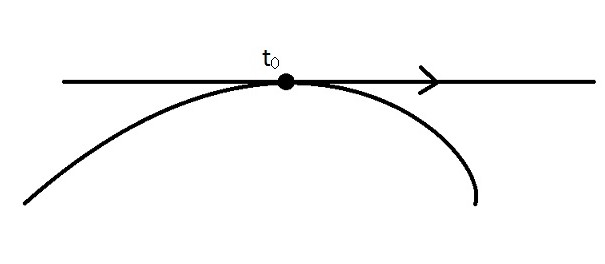
\includegraphics[width = 4.5cm]{tangent}

$\varphi' (t_0) \not = \vec 0$ - касательная прямая

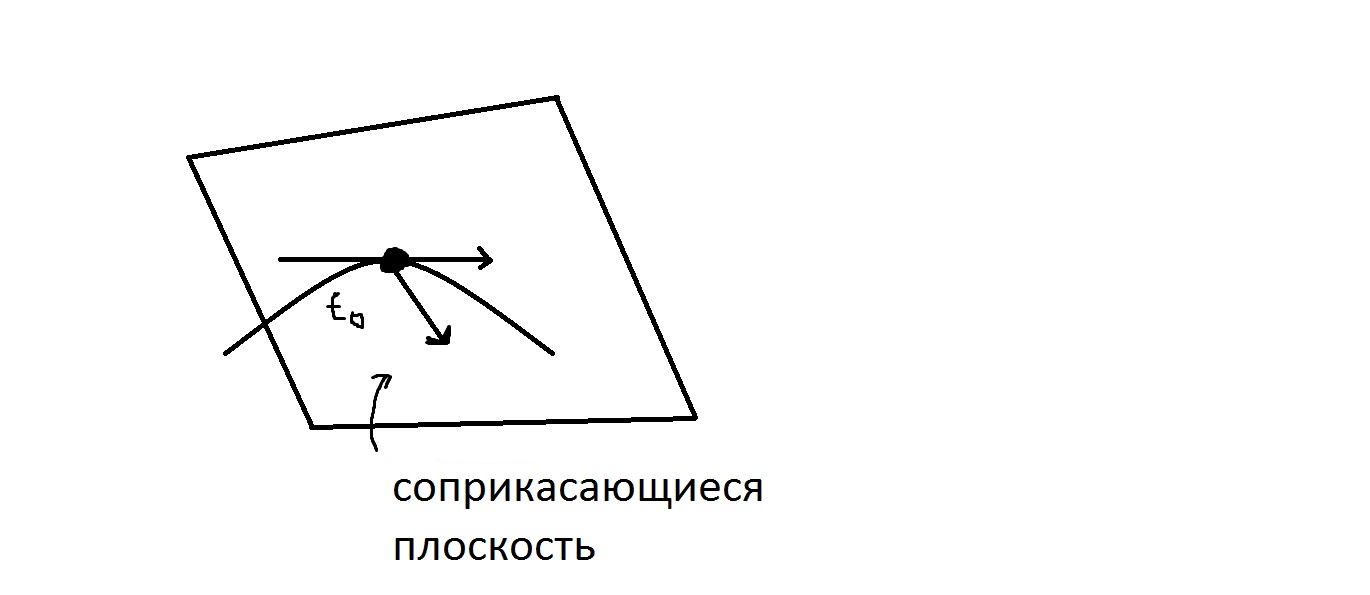
\includegraphics[width = 6cm]{beleg}

Соприкасающиейся  л.н.з (некомпланарная) плоскость.

$t_0$ называется точкой билигулярности.

$\vec \varphi = \vec p(t)$ называется билигулярной если все ее точки являются
точками билигулярности

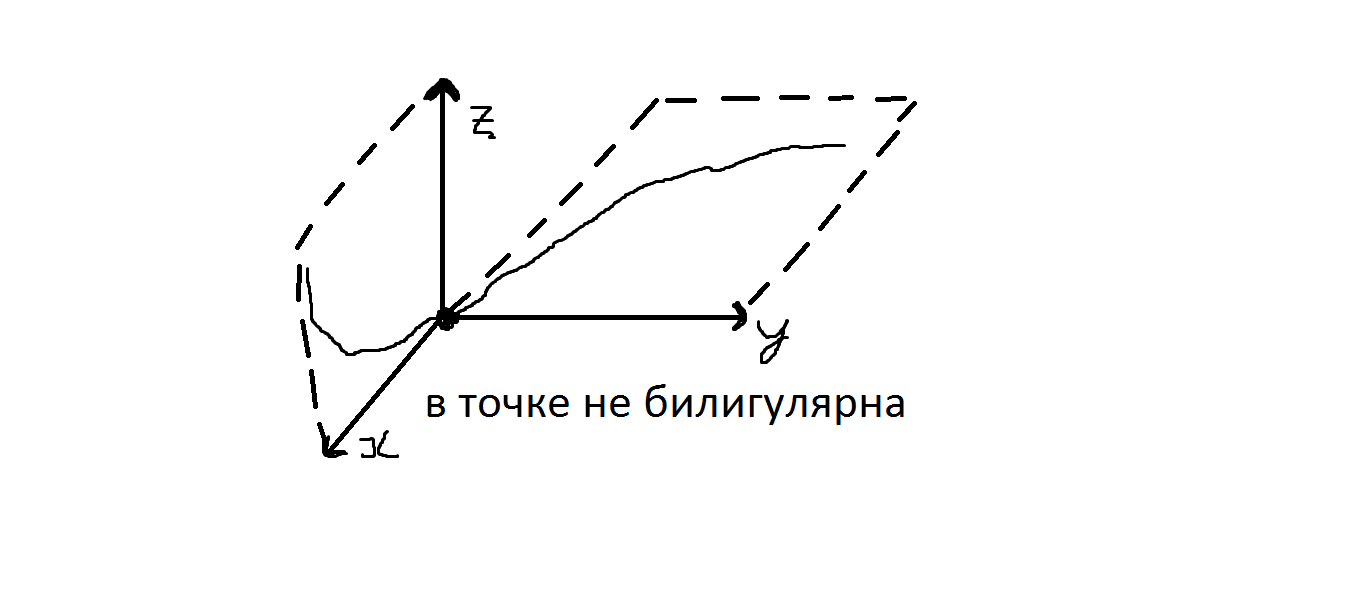
\includegraphics[width = 6cm]{notBeleg}

Пример:
$$
\left\{
\begin{array}{l}
x = a \cos t \\
y = a \sin t
\end{array}
\right.
s = \tg \frac{t}{2} ~~~ \sin t = \frac{2s}{1+s^2} ~~~
\cos t = \frac{1-s^2}{1+s^2} ~~~
\left\{
\begin{array}{l}
x = a \frac{1-s^2}{1+s^2} \\
y = a \frac{2s}{1+s^2}
\end{array}
\right.
$$

\begin{define}[диффеоморфизма]
  Диффеоморфизмом называется гладкое отображение при котором обратное
  отображение тоже гладкое.
\end{define}

Биективное отображение гладкое в обе стороны.

\begin{define}
  Пусть даны две кривые

  $\varphi_1 : [a,b] \to R^3$

  $\varphi_2 : [a,b] \to R^3$

  Эти кривые называются эквивалентными если существует диффeoморфизм
  $\varphi : [a,b] \to [\alpha, \beta]$
\end{define}

Пример:
$$
\varphi_1(t) = (a\cos t, a \sin t)
$$
$$
\varphi_2(t) = (a \frac{1-s^2}{1+s^2}, a \frac{2s}{1+s^2})
$$

Параметризация эквивалентных прямых называется эквивалентными если все кривые
разбиваются на классы эквивалентных кривых эти классы классы эквивалентности
кривых называются не параметрихованными кривыми.

\begin{theorem}
  Расмотрим множество оточек заданным соотнощением $F(x, y) = 0$ - гладкая
  функция. Пусть $\exists (x_0, y_0)$ такая что $F(x_0, y_0) = 0$ тогда
  $$
  \grad F(x_0, y_0) = \left( \frac{\partial F}{\partial x}(x_0, y_0);
  \frac{\partial F}{\partial y}(x_0, y_0) \right)
  $$
  тогда $\exists (x_0, y_0)$ в которой множество точек улидотворяет
  $F(x, y) = 0$ является образом регулярных кривых

  В этом случа мы будем говорить что это регулярная кривая задана неявно
  соотношением $F(x, y) = 0$.
\end{theorem}

\begin{theorem}[о неявных функциях]
  Пусть  даны гладкие функции
  $$
  \begin{array}{c}
    F_1 (x_1, x_2, \cdots, x_n, y_1, y_2, \cdots, y_n) \\
    \dots ~~~ \dots ~~~ \dots ~~~ \dots  ~~~ \dots ~~~ \dots \\
    F_m (x_1, x_2, \cdots, x_n, y_1, y_2, \cdots, y_n)
  \end{array}
  $$
  Тогда если точка $(x_0, y_0)$ такова что каждая функция в этой точке дает $0$
  и
  $$
  \left|
  \begin{array}{ccc}
    \frac{\partial F_1}{\partial y_1} & \dots &
    \frac{\partial F_1}{\partial y_1} \\

    \dots & \dots & \dots \\

    \frac{\partial F_m}{\partial y_1} & \dots &
    \frac{\partial F_m}{\partial y_m} \\
  \end{array}
  \right|
  \not= 0
  $$
  то $\exists O(x_0, y_0)$ в которой точки улидотворяющие соотношением
  $$
  \left\{
  \begin{array}{c}
    F_1(x, y) = 0 \\
    \dots ~~~ \dots \\
    F_m(x, y) = 0
  \end{array}
  \right. ~~~ \text{задаются} ~~~
  \left\{
  \begin{array}{c}
    y_1 = f_1(x_1, x_2, \cdots, x_n) = 0 \\
    \dots ~~~ \dots ~~~ \dots ~~~ \dots \\
    y_n = f_m(x_1, x_2, \cdots, x_n) = 0
  \end{array}
  \right.
  $$
  для некоторых гладких функций $f_1, f_2, \cdots, f_m $
\end{theorem}

\begin{proof}
  По условию  точка $(x_0, y_0)$
  $$
  \grad F(x_0, y_0) = \left( \frac{\partial F}{\partial x}(x_0, y_0);
  \frac{\partial F}{\partial y}(x_0, y_0) \right) \not= 0
  $$
  Можем считать что $\frac{\partial F}{\partial y}(x_0, y_0) \not= 0$ по
  теореме о неявной функции найдется такая точка $(x_0, y_0)$ в которой
  множество точек улидотворяющих $F(x, y) = 0$ задается соотношением $y = f(x)$
  тоисть состоит из точек вида $(x, f(x))$ следовательно это множество точек
  задается параметрически уравнением $\vec \varphi (t, f(t))$

  $\vec \varphi = (1, f'(x)) \not= 0$ следовательно кривая заданная этим
  уравнением регулярная.
\end{proof}

Покажем что для кривой неявно заданной соотношением $f(x, y) = 0$ вектор
градиента является нормалью (перпендикулярью касательной кривой) и направлен в
сторону выпуклости кривой.

По теореме наша кривая может быть задана параметрической кривой
$\vec \varphi = (x(t), y(t))$ тогда
$$
F(x(t), y(t)) = 0 ~~~
\frac{dF}{dt} = \frac{\partial F}{\partial x} \dots \frac{dx}{dt} +
\frac{\partial F}{\partial x} \dots \frac{dy}{dt} =
\grad F = 0 ~ \Rightarrow ~ \grad F \perp \varphi'
$$

\begin{title}[\Large]
  Параграф 2. Натурально параметрическая кривая, кривизна и кручение кривой
\end{title}

Пусть $\vec \varphi = \vec \varphi(t)$ - регулярная кривая, тогда длина дуги
кривой вычисляется по формуле
$$
S = \int_{t_0}^{t_1} | \vec \varphi'(t) dt
$$
если форма записи
$$
\left\{
\begin{array}{c}
  x = x(t) \\
  y = y(t) \\
  z = z(t)
\end{array}
\right.
S = \int_{t_0}^{t_1} \sqrt{ x'^2(t) + y'^2(t) + z'^2(t)}
$$

\begin{define}[натуральной параметризацией кривой]
  Параметризация при которой каждый точке кривой сопаставляется длина дуги кривой
  от точки до некоторой фиксированной точкой называется натуральной или
  естественной.
\end{define}

\begin{block}[Свойства]
  1) Натуральная параметризация эквивалентна исходной параметризации.

  \begin{proof}
    $\vec \varphi = \vec \varphi(t)$ - уравнение кривой

    $s = s(t)$ - натуральная параметризация
    $$
    \int_{t_0}^{t} |\varphi'(t)| dt ~~~
    \frac{ds}{dt} = |\varphi'(t)| > 0 ~ \Rightarrow ~ s = s(t) ~ \nearrow ~
    $$
    $\Rightarrow ~ s = s(t)$ является биективной
  \end{proof}

  2) $\left| \frac{d\varphi}{ds} \right| = 1$ для любой точки касательный
  вектор $= 1$

  \begin{proof}
    $\varphi(s) = \varphi (t(s))$

    $\frac{d\vec \varphi}{ds} = \frac{d\varphi}{dt} \frac{dt}{ds} =
    \vec \varphi' \cdot \frac{1}{|\varphi'|}$ вектор длины 1
  \end{proof}

  $$
  3) ~~~  \frac{d^2 \vec \varphi}{d^2 s} \perp \frac{d\vec \varphi}{ds}
  $$

  \begin{block}[Лемма]
    Если $|\varphi(t)| = const$, то утверждается что $\vec \varphi(t) \perp
    \vec \varphi(t)$
  \end{block}

  \begin{proof}
    $(\vec \varphi, \vec \varphi) = |\varphi|^2 = const$
  \end{proof}
  $$
  k =
  \left|
    \frac{d^2 \varphi}{d \xi}
  \right| ~~~
  \text{называется кривизной кривой}
  $$
  $$
    \frac{d^2 \varphi}{d \xi} ~~~ \text{вектор кривизны}
  $$
\end{block}

\begin{theorem}
  Кривизна кривой $= 0$ тогда когда ее образ является прямой
\end{theorem}

\begin{proof}
  $\Rightarrow$ Пусть $k = 0$ тогда $\left| \frac{d^2 s}{d^2} \right| = 0$
  $\frac{d^2 s}{d^2 s} = \vec 0$ $\frac{d s}{d s} = \vec a ~ (=const)$
  $\varphi = \vec a S + \vec b$

  прямая это $\varphi = c_0 + \vec g t$
\end{proof}